%=============================================================
% Header, Cover, and Preamble
%=============================================================
\documentclass[a4paper, 12pt, english]{book}
%=============================================================
\usepackage{amsmath} %use package here for formulas, maybe needed
\usepackage{graphicx} % This for Images
\usepackage{babel}
\usepackage{makeidx}
\usepackage{index}
\usepackage{datetime}
\usepackage{erewhon}
\usepackage{lipsum}
\usepackage{lettrine}
\usepackage{GoudyIn}
\usepackage[x11names]{xcolor} 
<<<<<<< HEAD
=======
\usepackage{indentfirst}
\usepackage{enumitem,amssymb}
\usepackage{listings}
\usepackage{tikz}
\usepackage{tikz-qtree}
\usetikzlibrary{trees}
\usepackage[a4paper, inner=1.7cm, outer=2.7cm, top=2cm, bottom=2cm]{geometry}

\newlist{todolist}{itemize}{2}
\setlist[todolist]{label=$\square$}
\usepackage{pifont}
\newcommand{\cmark}{\ding{51}}%
\newcommand{\xmark}{\ding{55}}%
\newcommand{\done}{\rlap{$\square$}{\raisebox{2pt}{\large\hspace{1pt}\cmark}}%
\hspace{-2.5pt}}
\newcommand{\wontfix}{\rlap{$\square$}{\large\hspace{1pt}\xmark}}



>>>>>>> dev
%=============================================================
\renewcommand{\LettrineFontHook}{\color{VioletRed4}\GoudyInfamily{}}
\LettrineTextFont{\itshape}
\setcounter{DefaultLines}{3}%
%=============================================================
\makeindex
%=============================================================
\title{\textbf{Software Engineering Project Report}}
%-------------------------------------------------------------
\newdateformat{monthdayyeardate}{
	\monthname[\THEMONTH]~\THEDAY, \THEYEAR}
%=============================================================
% Beginning of The Document
%=============================================================
\begin{document}
\author{Belal Hmedan \& Deng Jianning\\University Bourgogne}
%=============================================================
\maketitle
%=============================================================
\let\cleardoublepage\clearpage
%=============================================================
\tableofcontents
%=============================================================
% The Core of Report
%=============================================================
\chapter*{Introduction}
\addcontentsline{toc}{chapter}{Introduction} \markboth{INTRODUCTION}{}
<<<<<<< HEAD
\lettrine{B}{uilding} an Offline Map Software is a challenging project, because it requires a good knowledge in Geography, Mathematics, Graph Theory, and Computer Science.
\\At the very beginning of such project many questions must be asked, such as: \\Which places should the Map covers? For which application the Map will be used?
Which Information is necessary, and Which Information is useless so it can be \\Filtered, so total amount of Data will be reduced.
\\This Project is a try to answer some of many questions that any computer science Student will ask while starting this kind of projects. Maybe we didn't answer all The questions because of time limit, but we hope that this project will be useful For Other students to get some answers , and to get the fastest way between two Locations, That's why we selected 20 Locations carefully to satisfy the daily needs Of Students like Universities, Cool Restaurant, Pharmacy, Hospital, Shopping Centers, Students Residences, etc.
\\This project with all cool features and nice looking objects, is nothing more than "Hello Map", because Cartography is a great science developing everyday for both Civil and military use, and everyday there is changes on our planet leads to changes On the Map, starting from Environmental changes, and not ending by Human-Made changes. 
=======
\lettrine{B}{uilding} an Offline Map Software is a challenging project, 
because it requires a good knowledge in Geography, Mathematics, 
Graph Theory, and Computer Science.\\

At the very beginning of such project many questions must be asked, such as: 
What places should the Map covers? For which application the Map will be used?
Which Information is necessary, and which information is useless so it can be 
filtered, so total amount of Data will be reduced.\\

This Project is a try to answer some of many questions that any computer 
science Student will ask while starting this kind of projects. Maybe we 
didn't answer all The questions because of time limit, but we hope that 
this project will be useful For Other students to get some answers , and 
to get the fastest way between two Locations, That's why we selected 20 
Locations carefully to satisfy the daily needs Of Students like Universities, 
Cool Restaurant, Pharmacy, Hospital, Shopping Centers, Students Residences, etc.\\

This project with all cool features and nice looking objects, is nothing more 
than "Hello Map", because Cartography is a great science developing everyday 
for both Civil and military use, and everyday there is changes on our planet 
leads to changes On the Map, starting from Environmental changes, and not ending 
by Human-Made changes. 
>>>>>>> dev

%=============================================================
\chapter{Project Description}
%=============================================================
<<<<<<< HEAD
\section{Goal of the Project}
The goal of this project is to develop a software to locate (and rate) various buildings, such as schools, university buildings, major offices, hospitals, various shops, cool restaurants, streets, roads, parks, and other interesting points in Le-Creusot.
The key idea is to develop a software to visualize Le-Creusot, its streets, some
buildings, roads, and parks, in which the user can perform several actions, such as asking for an itinerary between two (or passing through more) points.
%=============================================================
\section{Completeness of the Project}
%-------------------------------------------------------------
\subsection{Place Locating}
Twenty locations were provided on this project, and there is ability to add many other places due to requirements, but user can't add places, only programmer.
User's privilege on this stage of the project is limited to chose only from a list of those twenty places.
% Deng can say something here.
%-------------------------------------------------------------
\subsection{Place Rating}
This Feature isn't added yet, but it maybe available in next releases.
%-------------------------------------------------------------
\subsection{Routing}
Routing in this stage only by foot, expanding travel Methods to car, bicycle, and Train is possible in the following releases. 
%=============================================================
\section{Dependencies}
Apart from STL, I’m using Boost Graph Library (BGL), which in turn depends on other Boost Library: Property Map, which in turn depends on other Boost Libraries, so I included the whole Boost Libraries at once.
\section{Data Sets Introduction}
=======
\section{Overview of the Project}

% \begin{enumerate}
% 	\item The first item
% 	\item The second item
% 	\item The third etc 
% \end{enumerate}

The goal of this project is to develop a software to show the whole picture of Le Creusot city. Apart from that, it also locates various amenities, such as schools, university buildings, major offices, hospitals, various shops, cool restaurants, streets, roads, parks, and other interesting points in Le-Creusot. With this map, user can search, rate and comment for the places of interests and do routing to get there. I the follow section, a more clear picture of the goals and achievements of this picture will be shown. \\

This project would be a great opportunity for us to practice and get a little bit more familiar with the C++. Besides, it's also a chance for us to project management. This two parts of contents will also be explain in the following.



\section{Dataset Introduction}

In this project, we decide to use OSM(open-street-map) data as the base data. OSM data provides huge amount of detailed but abstract details for users. We choose this dataset because the following advantages:

\begin{enumerate}
	\item  It provide detailed data base on nodes, ways and relations. Which will be more convenient to implement the Dijkstra's algorithms for routing.
\end{enumerate}

%=============================================================
\section{Completeness of the Project}
%-------------------------------------------------------------
% \subsection{Place Locating}

For this release of the application

\begin{enumerate}
	\item File I/O
		\begin{todolist}
			\item[\done] Loaded by the user
			\item[\wontfix] Modified and saved by the user
		\end{todolist}
	\item Map Displaying
	\begin{todolist}
		\item[\done] Graphically display the map 
	\end{todolist}
	\item Available Location
	\begin{todolist}
		\item[\done] Locations required in the reference is available
		\item[\done] Almost all locations contained in OSM data is available
	\end{todolist}
	\item Roads and routing 
	\begin{todolist}
		\item[\done] Presenting roads
		\item[\done] Different kinds of roads are distinguished graphically.
		\item[\done] Basic routing with 20 places as begining or end
		\item[\wontfix] Different travel mode
	\end{todolist}
	\item Offline
	\begin{todolist}
		\item[\done] All the features is based on offline OSM data
	\end{todolist}
\end{enumerate}

% % Twenty locations were provided on this project, and there is ability to add many other places due to requirements, but user can't add places, only programmer.
% % User's privilege on this stage of the project is limited to chose only from a list of those twenty places.
% % Deng can say something here.
% %-------------------------------------------------------------
% \subsection{Place Rating}
% This Feature isn't added yet, but it maybe available in next releases.
% %-------------------------------------------------------------
% \subsection{Routing}
% Routing in this stage only by foot, expanding travel Methods to car, bicycle, and Train is possible in the following releases. 
% %=============================================================




\section{Dependencies}

\begin{enumerate}
	\item {\textbf{Boost}}\\
	Need to be installed if you don't have it. Follow the installation guide below.
		\begin{itemize}[noitemsep]
		\item {\textbf{Windows}} \\
		\item {\textbf{Ubuntu}} \\
		If it is not pre-install in your Ubuntu, a single command 
		should help you do this (for Ubuntu 18.04):
		\begin{lstlisting}[language=bash]
$ apt-get install libboost-all-dev
		\end{lstlisting}
		\end{itemize}
	\item {\textbf{Libosmium}} \\
		This is a header-only library, no need for installation. 
		Just includ the header files in the project is OK to go.
		This is already put in the project repository.
	\item {\textbf{Protozero}} \\
		This is a header-only library, no need for installation. 
		Just includ the header files in the project is OK to go.
		This is already put in the project repository.
	\item {\textbf{Zlib}} \\
	Need to be installed if you don't have it. Follow the installation guide below.
		\begin{itemize}[noitemsep]
		\item {\textbf{Windows}} \\
		\item {\textbf{Ubuntu}} \\
		If it is not pre-install in your Ubuntu, a single command 
		should help you do this (for Ubuntu 18.04):
		\begin{lstlisting}[language=bash]
$ apt-get insatll zlib1g-dev
		\end{lstlisting}
		\end{itemize}
	\item {\textbf{Expat}}\\
	Need to be installed if you don't have it. Follow the installation guide below.
	\begin{itemize}[noitemsep]
	\item {\textbf{Windows}} \\
	\item {\textbf{Ubuntu}} \\
	If it is not pre-install in your Ubuntu, a single command 
	should help you do this (for Ubuntu 18.04):
	\begin{lstlisting}[language=bash]
$ apt-get insatll expat
	\end{lstlisting}
	\end{itemize}
	\item {\textbf{PThread}} ( for Linux ) \\
	Use the following command to install the library
	sudo apt-get install libpthread-stubs0-dev
	\begin{lstlisting}[language=bash]
$ apt-get insatll expat
	\end{lstlisting}
	% \end{itemize}
	
\end{enumerate}

% Apart from STL, I’m using Boost Graph Library (BGL), which in turn depends on other Boost Library: Property Map, which in turn depends on other Boost Libraries, so I included the whole Boost Libraries at once.
% \section{Data Sets Introduction}







>>>>>>> dev
%=============================================================
\chapter{Code Design and Structure}
%\section{Overview}




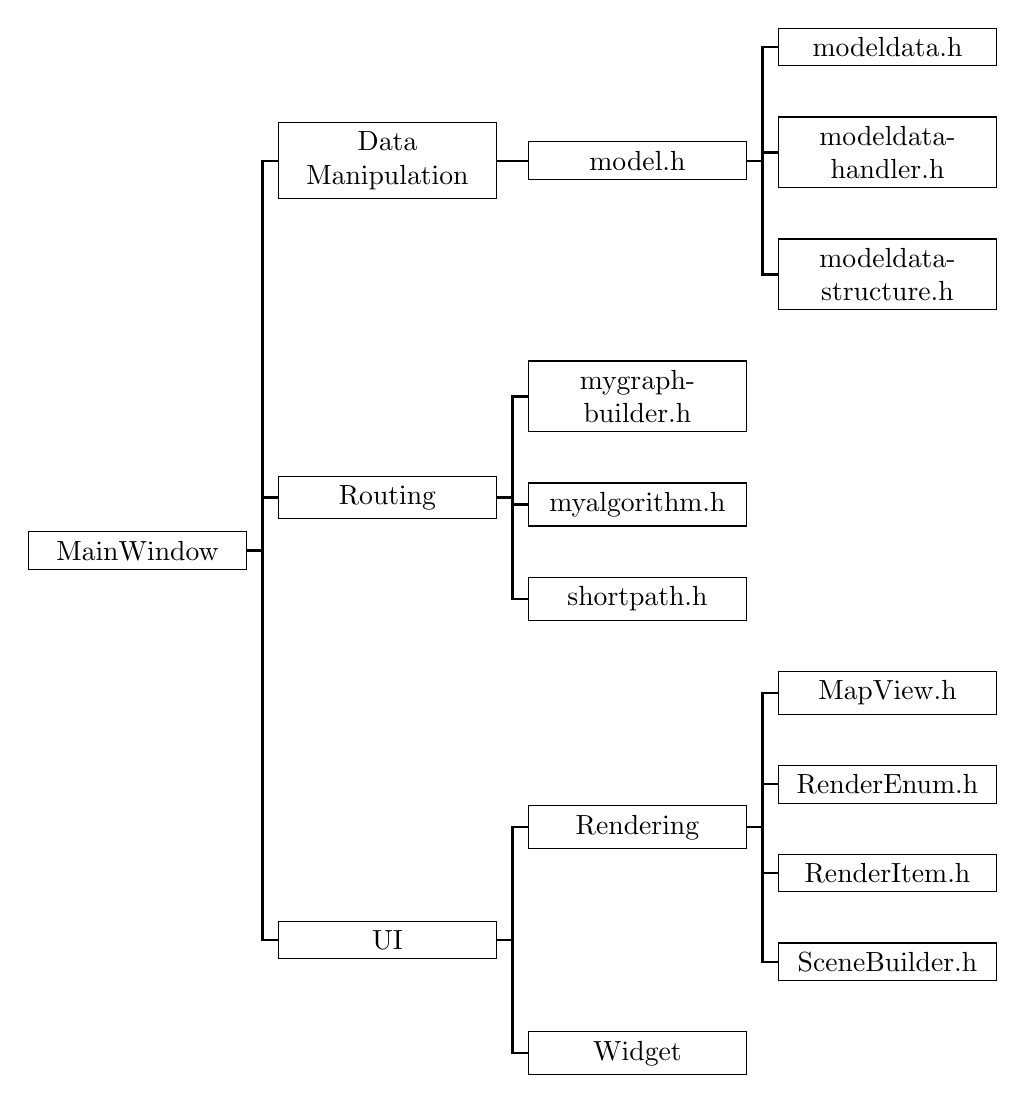
\begin{tikzpicture}[grow'=right,level distance=1.25in,sibling distance=.25in]
\tikzset{edge from parent/.style= 
	{thick, draw, edge from parent fork right},
	every tree node/.style=
	{draw,minimum width=1in,text width=1in,align=center}}
\Tree 
[. MainWindow 
	[.{Data\\Manipulation}
		[.{model.h } 
			[.{modeldata.h } ]
			[.{modeldata-\\handler.h } ]
			[.{modeldata-\\structure.h } ]
		]
	]
	[.{Routing}
		[.{mygraph-\\builder.h} ]
		[.{myalgorithm.h} ]
		[.{shortpath.h} ]
	] 
	[.{UI} 
		[.{Rendering } 
			[.{MapView.h} ]
			[.{RenderEnum.h} ]
			[.{RenderItem.h} ]
			[.{SceneBuilder.h} ]
		]
		[.{Widget } ]
	]
]
\end{tikzpicture}
\\
%=============================================================
\section{Data Manipulation}

%=============================================================
\section{Algorithm and Routing}

This part of code organized in 3 different Classes, each of them contains Header, and Source File:
%-------------------------------------------------------------
\subsection{ MyGraphBuilder Class:}
This Class mainly handles data provided from our Data Structure represented by the Model which depends on the OSM file in its compressed format PBF.
This Class mainly takes the nodes included inside ways only from the
Model as an input, then builds Vertices and Edges Between Vertices to construct the Graph, which in turn will be as an input to the Next stage which is Dijkstra Algorithm.
The Graph in my approach is Adjacency List proposed by Boost Graph Library.
The need for this procedure comes from the fact that: finding shortest path will be implemented through an algorithm, and the algorithm deals with graph, so I wrote this class to build the desired Graph from the Data Structure we imported from OSM file.
The input for this Class is the Model (Data Structure) extracted from OSM file, 
And the Output is a Bidirectional weighted Graph.
Bidirectional, because it’s easy to implement, in case we want improve it to Directional Graph, we must do a complicated constrains, and check each Tag, to see the type of Transportation, and if the way was one direction, or bidirectional.
Weighted Graph: because we are calculating Euclidean Distance between the Nodes depending on Longitude, and Latitude.
%-------------------------------------------------------------
\subsection{ MyAlgorithm Class:}
This Class takes the Graph produced on the past class MyGraphBuilder, and the Source Node which we will start from, and runs Dijkstra Algorithm proposed by Boost Graph Library to Find the Shortest Path Between the Source Node, and all other Nodes in The Graph.
Special Function in this class called: getShortPath takes the destination Node, then returns the shortest path between the source and destination only.
In case that there was no path between nodes, the path (Vector) will contain only one default node, so we don’t face issues due to empty vector.
%-------------------------------------------------------------
\subsection{ ShortPath Class:}
This Class is just to reduce amount of code in the main window, it doesn’t do much, it just takes Source Node, Destination Node, and Model, then it builds the Graph From the Model using MyGraphBuilder Class, and Runs MyAlgorithm Class, and its special Function getShortPath, finally the output is our shortest path.



%=============================================================
<<<<<<< HEAD
\section{Data Manipulation}

%=============================================================
\section{Rendering}

%============================================================
\section{Routing}
Routing on this approach is just on foot, it’s possible to add more transport methods later using Tag filtering, building different transport maps, Vertices, and Edges, but unfortunately time was short for this project ! .
Isolated Nodes which doesn’t belong to any way are not included in building the Graph, because our purpose is to find a way between two nodes, so I didn’t build the graph with all nodes, only connected nodes which belong to way.
Euclidean Distance between the Nodes is our way to assign weight to Edges between Nodes, and of course the Way or Path is nothing except group of sequential Edges between connected Nodes.
=======
% \section{Routing}
% Routing on this approach is just on foot, it’s possible to add more transport methods later using Tag filtering, building different transport maps, Vertices, and Edges, but unfortunately time was short for this project ! .
% Isolated Nodes which doesn’t belong to any way are not included in building the Graph, because our purpose is to find a way between two nodes, so I didn’t build the graph with all nodes, only connected nodes which belong to way.
% Euclidean Distance between the Nodes is our way to assign weight to Edges between Nodes, and of course the Way or Path is nothing except group of sequential Edges between connected Nodes.
>>>>>>> dev
%============================================================
\section{GUI}
\subsection{Rendering}




\subsection{Widget}
Running the Program that will show a window with a Menu and four buttons Source, Destination, Navigate, and Cancel.
%------------------------------------------------------------
\begin{center}
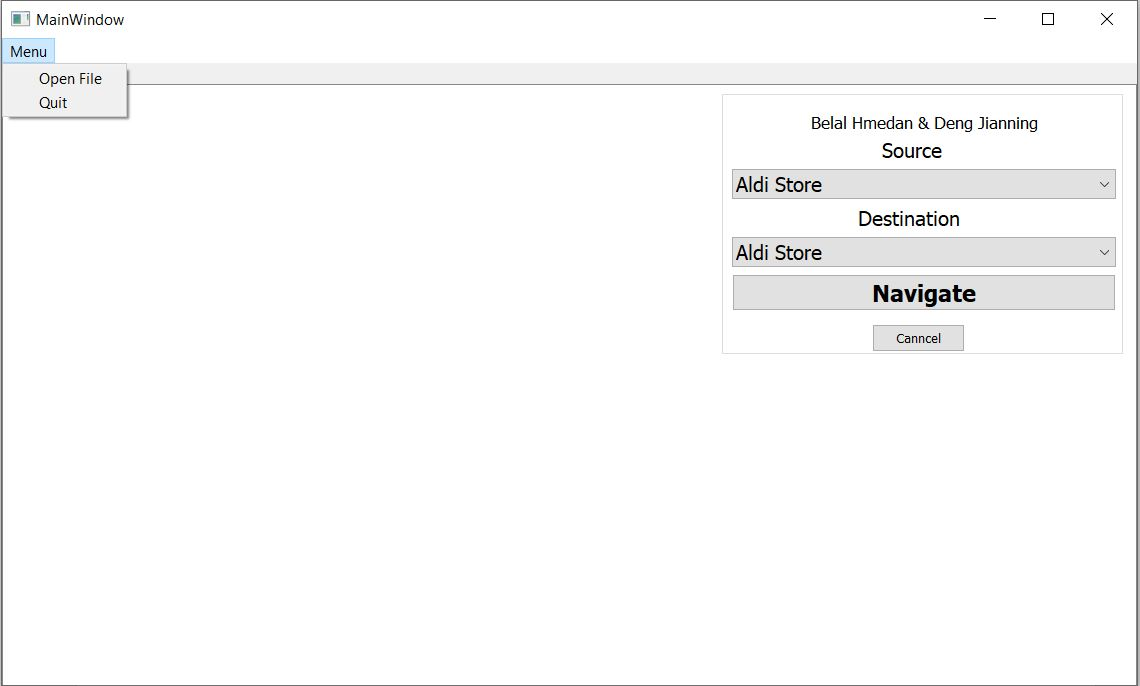
\includegraphics[width=.6\textwidth]{GUI_NoMap.JPG}
%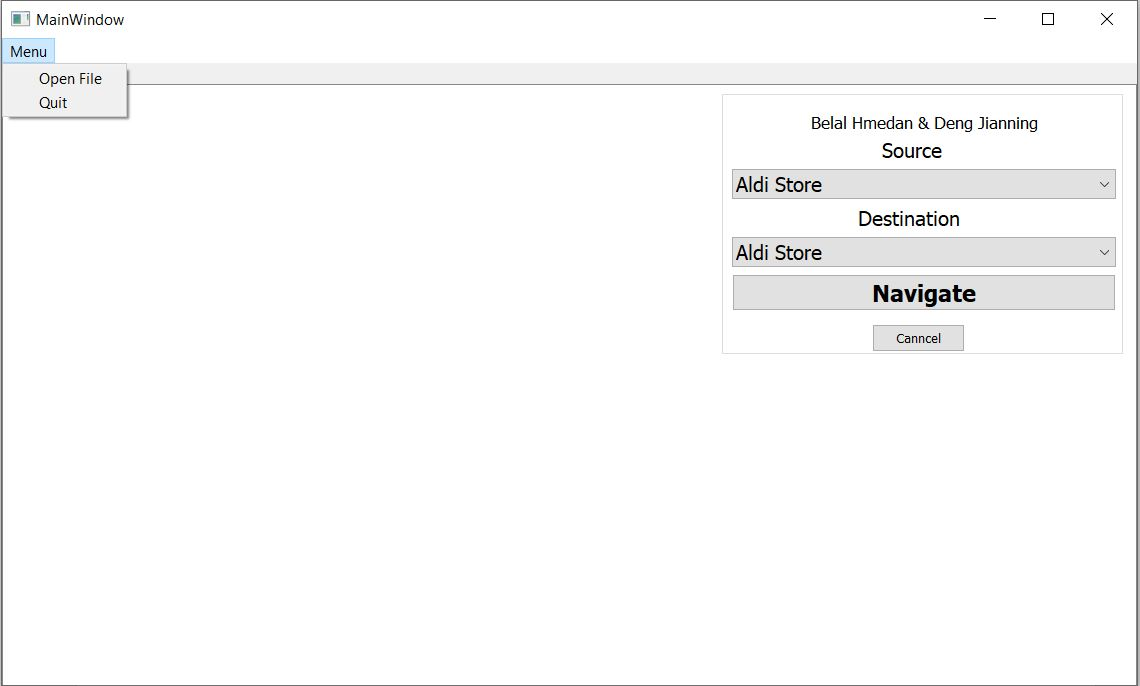
\includegraphics[width=.6\textwidth,natwidth=1200,natheight=700]{GUI_NoMap.JPG}
\end{center}
%------------------------------------------------------------
To start working, you should select (Menu - Open )
to open the map file, which should be with (.pbf) extension.
After you select your Map, the Software loads the map File showing the Map.
%------------------------------------------------------------
\begin{center}
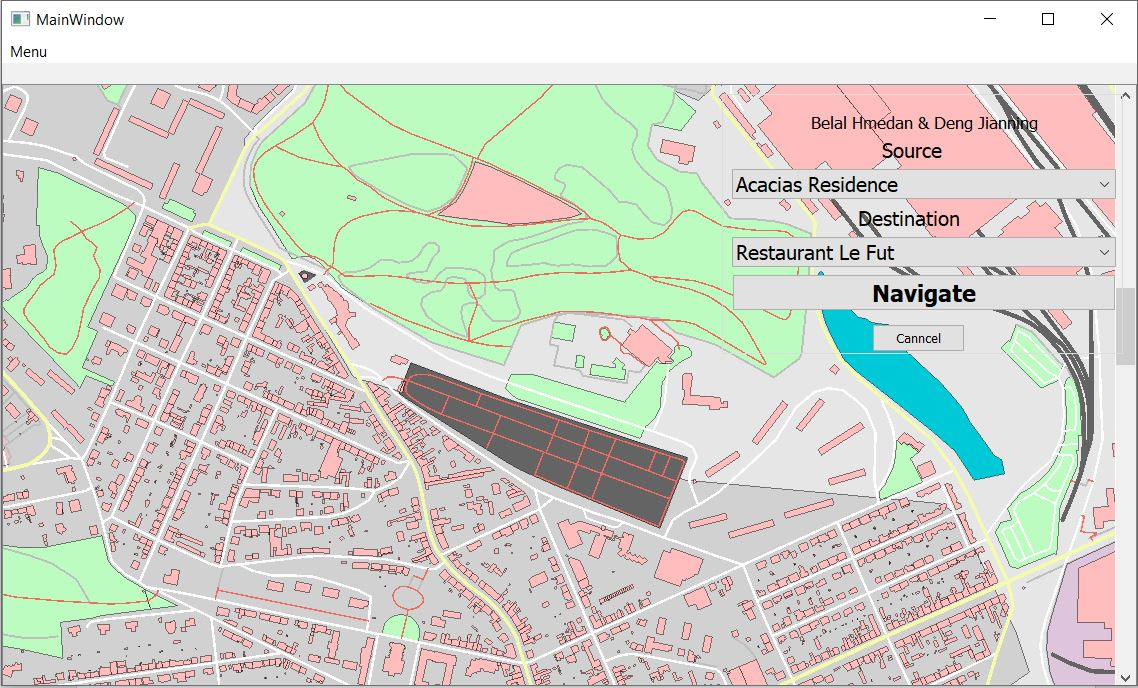
\includegraphics[width=.6\textwidth]{GUI_Map0.JPG}
%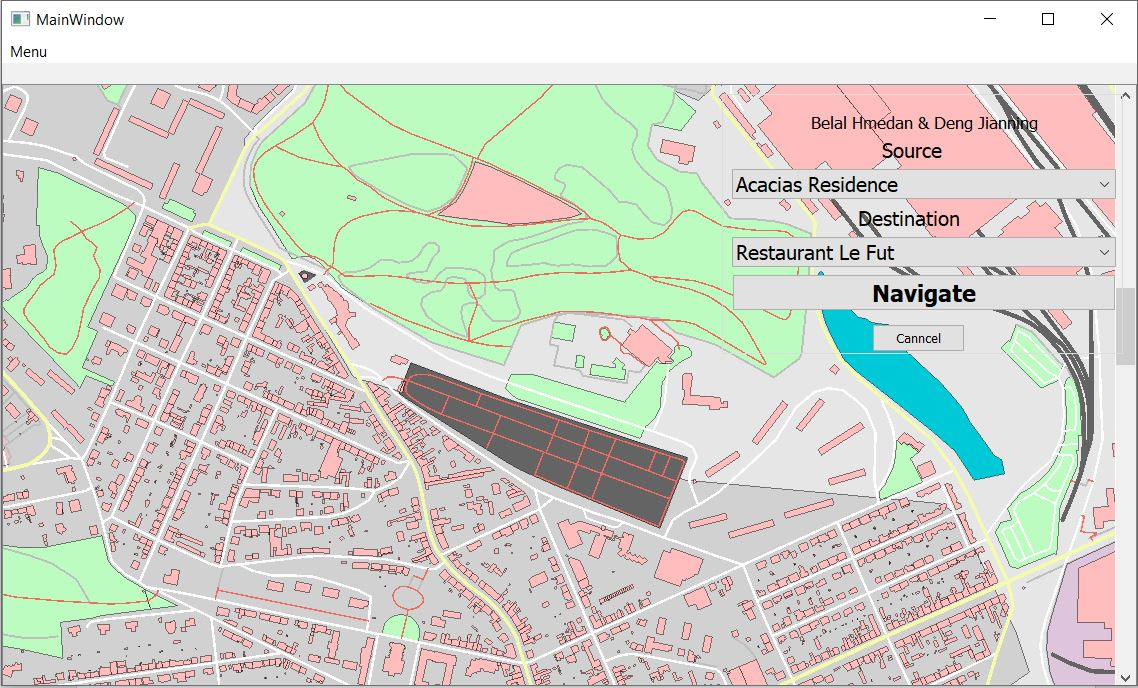
\includegraphics[width=.6\textwidth,natwidth=1200,natheight=700]{GUI_Map0.JPG}
\end{center}
%------------------------------------------------------------
The Drop-down lists Source, and Destination contains 20 places for each of them, All on Le Creusot City, where you can select your start point, and destination.
%------------------------------------------------------------
\begin{center}
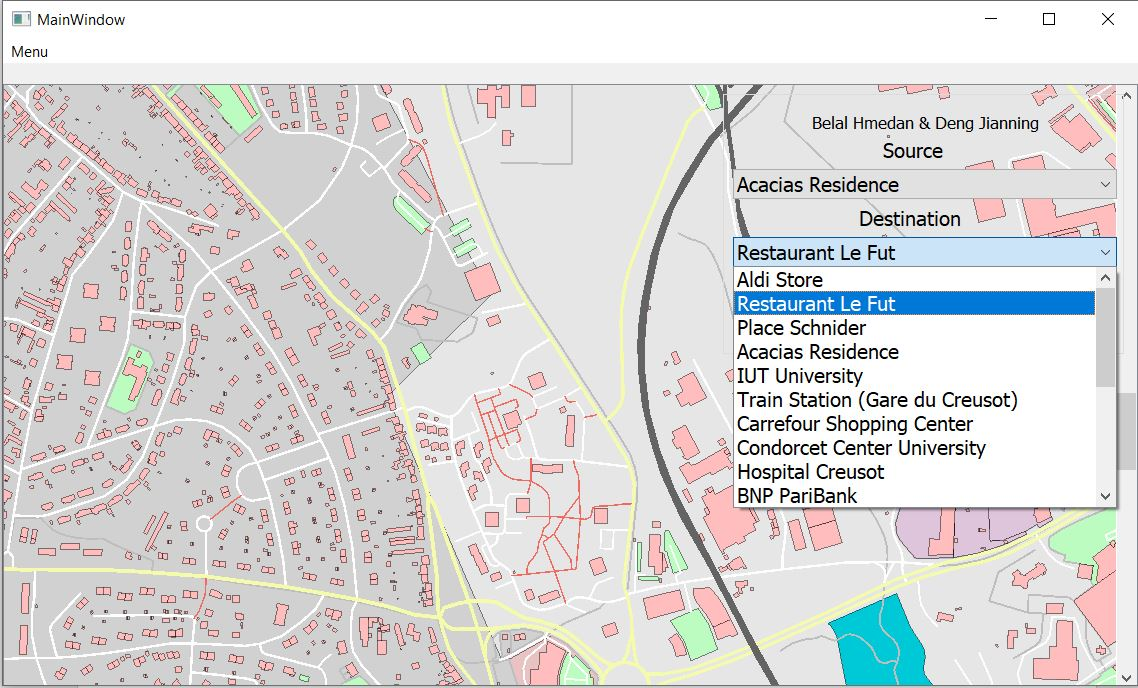
\includegraphics[width=.6\textwidth]{GUI_Map1.JPG}
%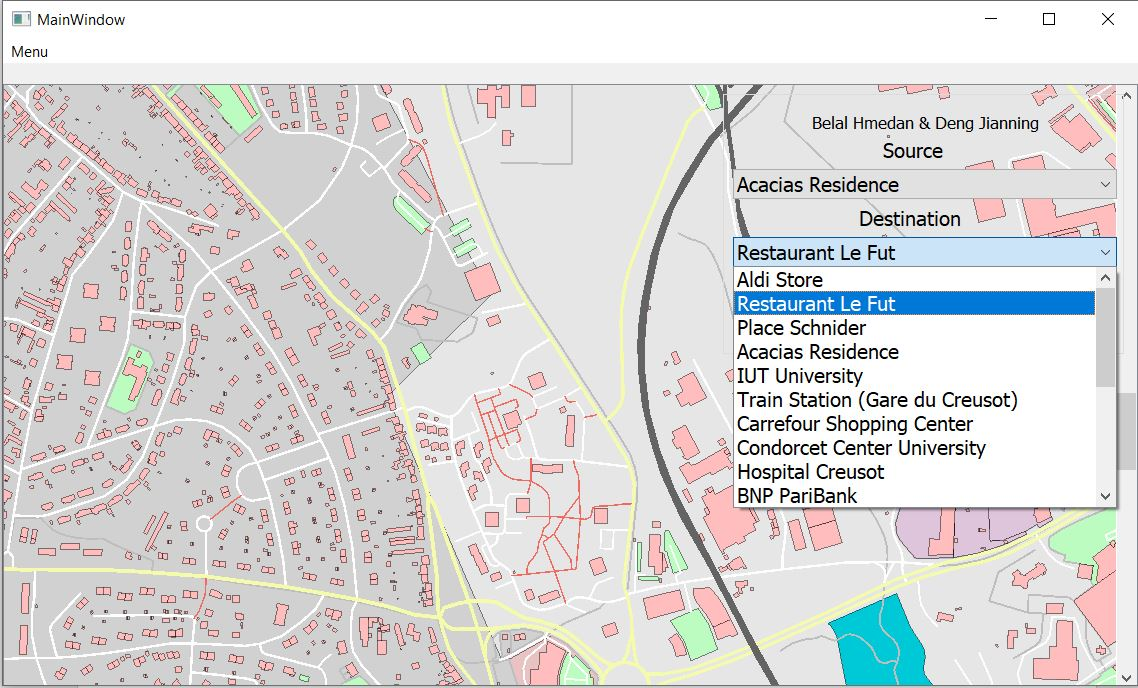
\includegraphics[width=.6\textwidth,natwidth=1200,natheight=700]{GUI_Map1.JPG}
\end{center}
%------------------------------------------------------------
by clicking on Navigate Button, the Shortest Path will be drawn by Red , so you can see the way you should follow.
%------------------------------------------------------------
\begin{center}
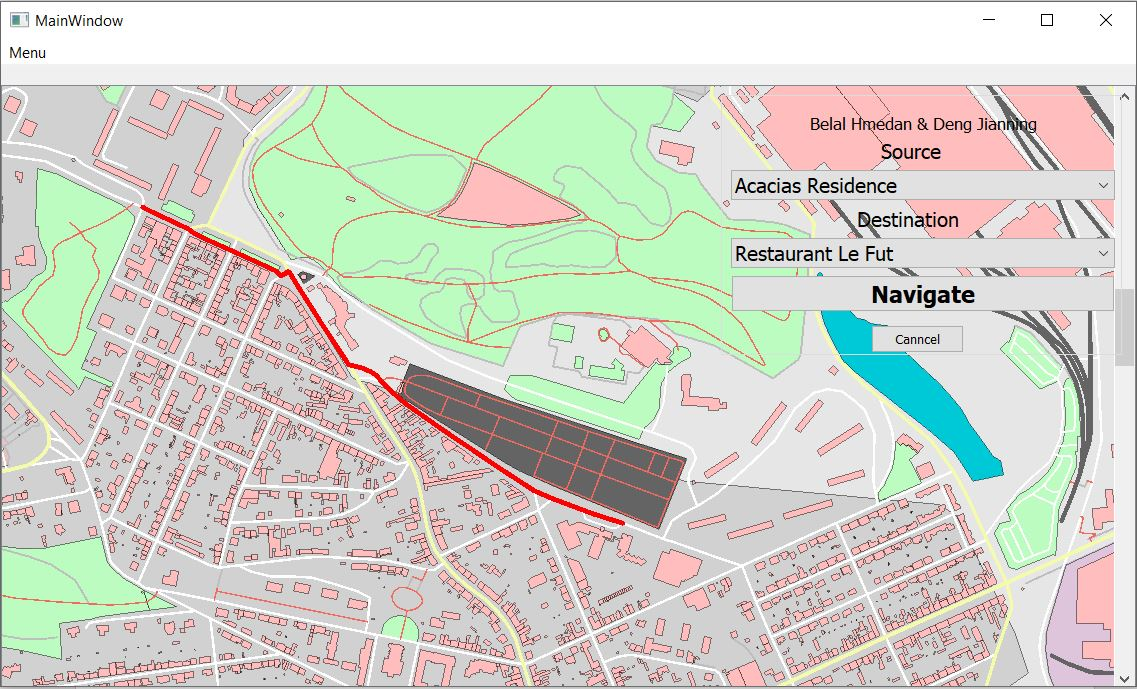
\includegraphics[width=.6\textwidth]{GUI_Map2.JPG}
%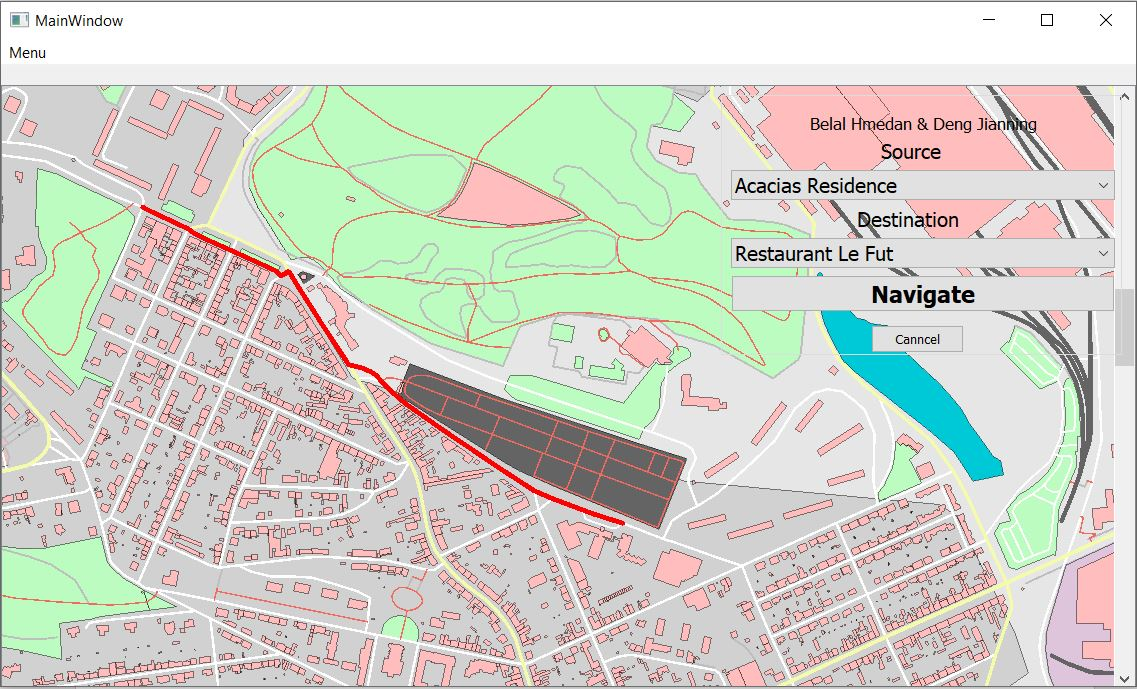
\includegraphics[width=.6\textwidth,natwidth=1200,natheight=700]{GUI_Map2.JPG}
\end{center}
%------------------------------------------------------------
Cancel button is to hide that path, and you can choose again your start point and target, so your path again will be drawn for you.
To Finish, you can select (Menu - Quit) to exit the Software.





%=============================================================
\section{Difficulties during implementation:}
There is two kind of Difficulties here:
%-------------------------------------------------------------
\subsection{Difficulties we got rid of it:} 
%*************************************************************
\subsubsection{First Difficulty was CMake didn’t find some libraries:}
specially Boost Library, later we excluded Cmake, we depended on Headers only to implement our plan.
%*************************************************************
\subsubsection{Second Difficulty was that Edges can’t be built using idType Nodes:} the solution for that was mapping the idType Nodes to unsigned int indexes through a map, so each node has ID, and Vertex Number.
%*************************************************************
\subsubsection{Third one is Redundancy of Nodes in different Ways:} the solution was to compare each node of way to the map we built as solution to problem1.2, so if the node already found, we don’t add it to our map, instead we just call it and get Node index.
%-------------------------------------------------------------
\subsection{Difficulties we can solve, but it needs more time:}
%*************************************************************
\subsubsection{1.Supporting Different Travel Method.}
%*************************************************************
\subsubsection{2.Building Directional Graph instead of Bidirectional one.}
%*************************************************************
\subsubsection{3.Adding Reviews, and stars options to the GUI.}
%*************************************************************
\subsubsection{4.Adding locations on the Map.}
%-------------------------------------------------------------
\subsection{Unexpected Difficulties}
Losing member of the team at critical time of the project doubled the responsibilities to do more than what we have already planned to do, and make us work under pressure in some parts of the project which we didn't have ideas about it before.
%=============================================================
\chapter{Project Management}
%=============================================================
\section{Overview of the Project Planning}
<<<<<<< HEAD
We Received the Project on 30Th of September,it took us about 2 weeks to team up in a group of 3 students, then we started The Research for the Project since 15Th of October, Research for this project took 3 weeks until 6Th of November, There was many choices, and due to strict conditions such as: the Project should work under different operating systems, we excluded promising solutions such as "Libsmscout" which was easy to use Library with advanced features, but it doesn't work on Windows, only Linux, that lead us to more complicated choices such as "Libosmium" and "Boost" Libraries.
=======
We Received the Project on 30Th of September,it took us about 2 weeks to 
team up in a group of 3 students, then we started The Research for the 
Project since 15Th of October, Research for this project took 3 weeks 
until 6Th of November, There was many choices, and due to strict conditions such as: the Project should work under different operating systems, we excluded promising solutions such as "Libsmscout" which was easy to use Library with advanced features, but it doesn't work on Windows, only Linux, that lead us to more complicated choices such as "Libosmium" and "Boost" Libraries.
>>>>>>> dev
The Implementation started on the 6Th of November, each student worked on different part of the project: "Data Manipulation and Map Rendering" for Deng, "Shortest Path Algorithm" for Belal, and "Graphical User Interface" for Our Third Partner.
Ten Days later At 16Th of November Deng Proposed Three Solutions for dealing with the Project:
\\ \textbf{}Solution 1: Using one-for-all library.
\\ \textbf{}Solution 2: Using OSM data access library.
\\ \textbf{}Solution 3: Display the map using Image.
At that Point Belal and Deng Agreed on the Second Solution, because we want to propose something different and more advanced than the Image.
Our Partner preferred to go on different Direction with Image Solution, so we had to work on the project as a team of two members only !.
Following the advice to "Expect what is Unexpected " we reduced the project size and features so we can finish it before Deadline.
A week later, on 24Th of November we had our first working project with Minimum features available, a week later on the 1st of December We did a simple GUI to deal with our Map.
Writing The Documentation took a week until 7Th of December, and Writing the Report in Latex took another week up to 14Th of December, so We did it on time.

%-------------------------------------------------------------
<<<<<<< HEAD
\section{Work Schedules}
%*************************************************************
=======



\section{Work Schedules}
%*************************************************************





>>>>>>> dev
\subsection{Plans VS Actual}
%-------------------------------------------------------------
\section{Conclusion}
%=============================================================
\chapter{Summary}
%=============================================================
\begin{thebibliography}{12}
\bibitem{BGL} 
Jeremy G. Siek,
Lie-Quan Lee, Andrew Lumsdaine.
\textit{The Boost graph library : user guide and reference manual.} , ``Book," \emph{BGL}, pp. 161-322,Pearson Education, Inc., Reading, Massachusetts, 2002.
\end{thebibliography}
%=============================================================
\end{document}